\documentclass[english,a4paper,twoside]{article}
\usepackage{autiwa}
\usepackage{aas_macros}

\title{Nautilus Documentation}
\author{Christophe Cossou, Maxime Ruaud, Valentine Wakelam}

\newcommand{\raccourci}[1]{{\bfseries #1}}
\newcommand{\molecule}[1]{\ensuremath{\mathrm{#1}}}

\lstset{commentstyle=\ttfamily\color{gray}}

\makeindex
\begin{document}

\begin{titlepage}
\begin{center}
~
\vfill
% Upper part of the page
\begin{figure}[t]
\centering
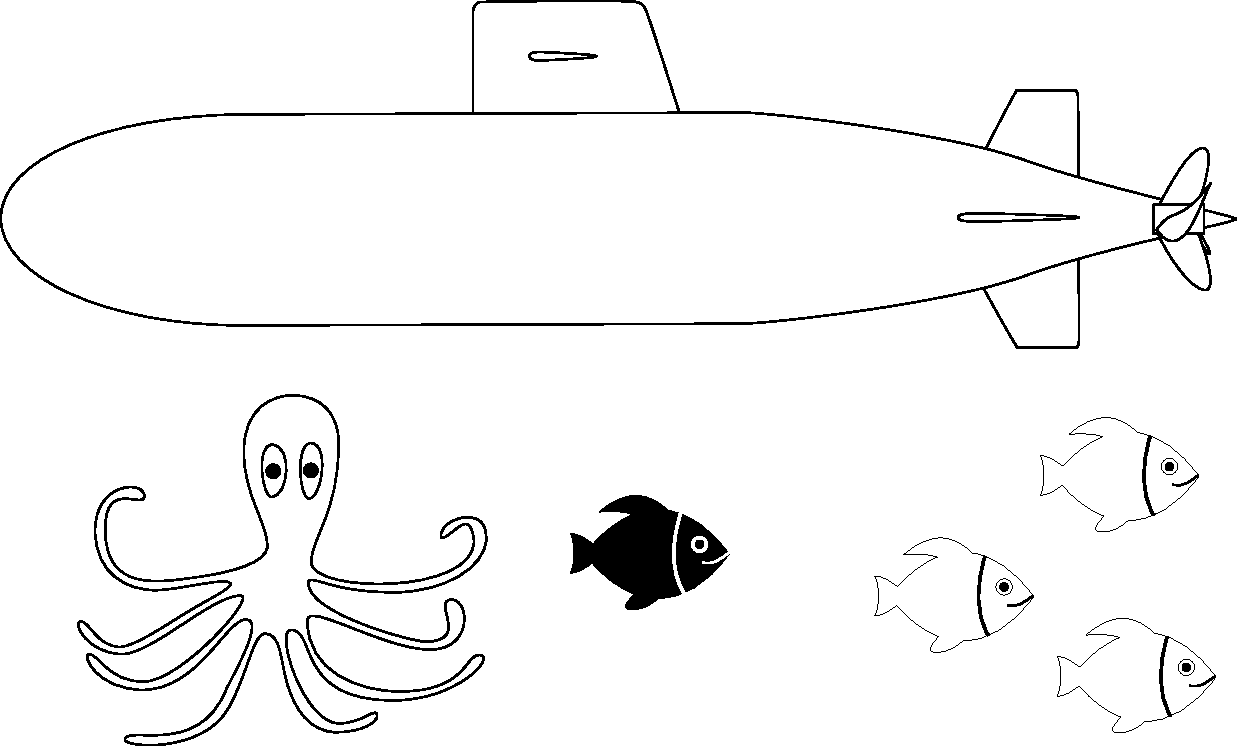
\includegraphics[width=0.5\textwidth]{figures/nautilus_logo.pdf}%chemin absolu de l'image pour que l'on puisse appeler ce fichier depuis plusieurs dossiers différents.
\end{figure}

% Title
\HRule \\[0.4cm]
{ \huge \bfseries \makeatletter\@title\makeatother}\\[0.4cm]

\HRule \\[0.75cm]
{\large \today}\\[0.75cm]
\makeatletter
\@author
\makeatother
\vfill
\vfill
~
% Bottom of the page


\end{center}
\end{titlepage}

\cleardoublepage

\tableofcontents

\cleardoublepage

\section{TODO}
\begin{itemize}
\item More details on \verb|grain_tunneling_diffusion| flag need to be added by someone who understand it
\item More details on \verb|modify_rate_flag| flag need to be added by someone who understand it
\item More details on \verb|conservation_type| flag need to be added by someone who understand it.
\item idem for \verb|is_absorption|
\item Reference for cosmic ray ionization rate standard value?
\item What is the reference UV flux? Paper describing it?
\item X ionization rate set to 0, is it normal?
\end{itemize}

\section{Starting with Nautilus}\label{sec:starting}
Whether you are a developer or a user, you do not have the same expectations about this manual. 

\refsec{sec:starting} explains the basics, mainly how to get the repository, how to compile the simulation code, how to use the various tools. Be sure to read carefully the section about \textbf{Installation} \refsec{sec:installation}.

\refsec{sec:chemical-network} explains the chemical network, its format, and the various types of reactions available. A chemical network is given with the code, but you can use your own. 

Input files are presented in \refsec{sec:input-files}, but the most important one, the only one you will modify daily (\gras[input file!parameters.in]{parameters.in}) is dealt with in \refsec{sec:parameters_in}.

Output files are presented in \refsec{sec:output-files}. Simulations information are displayed in \gras[output file!info.out]{info.out} (see \refsec{sec:info-out}).

\refsec{sec:graphic-display} explain what are the Python scripts you can use to plot useful information (mainly abundances) of your simulations (single plot or comparison between several runs).

One last section \refsec{sec:advanced} present technical specifications of the code and how to maintain it. For developers who wants more detailed explanations about the code, please refer to the Doxygen documentation, available in the Git repository at \url{http://nautilus.googlecode.com/git/html/index.html} or in the \textbf{html} repository of any local Git clone.

\subsection{Generic informations}
\subsubsection{Python scripts help}\label{sec:python-help}
From all the python script that come with the code, you can see all parameters and sometimes a few examples by typing:
\begin{verbatim}
script_name.py help
\end{verbatim}

\subsubsection{Comments in input files}\label{sec:files_generic_info}
For all input files, the comment character is " !" and can be either at the beginning of a line, or anywhere else. Meaningful character must be comprised inside the 80 first characters of a given line.

\subsubsection{Main parameter file}
\gras[input file!parameters.in]{parameters.in} is the main parameter file, and is rewritten by the code itself each and every time you run the code. 

\subsection{Getting the Git repository}
First, you need to get the Git repository from \gras{Googlecode} before actually using the code. 

I assume you only want to use it, without ever putting on the distant repository anything. This way, you don't even need to have an account and a password. 

In the parent directory where you want to put a \textbf{nautilus} folder containing the Git repository, type:
\begin{verbatim}
git clone https://code.google.com/p/nautilus/
\end{verbatim}

Be sure to run once in a while the command to get distant \gras[update]{updates} if they exists:
\begin{verbatim}
git pull
\end{verbatim}\index{git pull}\index{update}

\subsection{Installation}\label{sec:installation}
Once you have the Git repository, I advice you to run the script \gras{configure\_nautilus.py} : 
\begin{verbatim}
configure_nautilus.py
\end{verbatim}

This script will add useful shortcuts in the \gras{.bash\_profile}. When updating your Git repository, the bash commands will also be updated automatically into the \gras{.bash\_profile}.

\begin{attention}
Nautilus is a file browser in GNU/Linux (Gnome) environments. Thus, You must be \emph{very} careful. 

If you use:
\begin{verbatim}
nautilus
\end{verbatim}
in a terminal, you will not run the nautilus code, but rather the file browser (which you do not want, especially in a remote server, I assure you). 
\end{attention}

The improvements brought by this script are:
\begin{itemize}
\item You can go to the Nautilus folder by typing:
\begin{verbatim}
cd $nautilus
\end{verbatim}
\item You can launch the code, the output code and the rates code by these three commands, regardless of the folder you currently are:
\begin{verbatim}
nautilus_code
nautilus_outputs
nautilus_rates
nautilus_major_reactions
\end{verbatim}
\item You have now useful information about Git repositories directly into the Bash prompt.
\item all scripts in the folder \textbf{scripts/} can be run from any folder. This include:
\begin{verbatim}
nautilus-clean.sh # Cleaning a simulation folder
nautilus-plot-abundances.py # plot abundances of a simulation
nautilus-compare-abundances.py # compare two simulations or more.
\end{verbatim}
\end{itemize}

\begin{remarque}
All of this will have little interest for you if you don't use 'Bash' as the interpreter for you terminal.

You can also check the options of this script. Especially, you can undo the installation.
\end{remarque}

\subsection{Compilation}
The script \gras{Makefile.py} allow you to compile the code (see \refsec{sec:python-help} for infos about Python scripts). The default compiler is \gras{gfortran}. 

If you want to just compile the code\footnote{By default, all the binaries are compiled}, type:
\begin{verbatim}
Makefile.py
\end{verbatim}

\begin{remarque}
Errors are in \textbf{*.log} files associated with the module incriminated. Warnings are stored in a generic file \gras{compilation.log}.
\end{remarque}

\begin{attention}
By default, all warnings issued by \gras{ODEPACK} routines are masked (to increase readability, since nobody can modify this thing from scratch). An option \textbf{opkd} can force their display.
\end{attention}

If you want to compile \emph{only} one binary, use respectively those command:
\begin{verbatim}
Makefile.py nautilus
Makefile.py output
Makefile.py rates
Makefile.py major
\end{verbatim}

\bigskip

One particular option exist:
\begin{verbatim}
Makefile.py test
\end{verbatim}
This option \textbf{test} use compilation options that allow comparison of the code between different versions and is to be used for \gras{compare\_simulations.py} (see \refsec{sec:compare_simulation}). 

\begin{remarque}
Mainly, this option avoid too hard optimization that can result in slightly different results when the code evolve (not because the maths changes but because of optimization only).
\end{remarque}

Finally, one option exist so that you can compile one particular source file of the current working directory:
\begin{verbatim}
Makefile.py name=source_code.f90
\end{verbatim}
The Binary name will be \verb|source_code|

\begin{attention}
If you change compilation options, pay attention to use the option \textbf{force} to ensure all the modules will be compiled using these options.
\end{attention}

\subsection{Binaries}
The various binaries available are:
\begin{itemize}
\item \gras[binary!nautilus\_code]{nautilus\_code}
\item \gras[binary!nautilus\_outputs]{nautilus\_outputs}
\item \gras[binary!nautilus\_rates]{nautilus\_rates}
\item \gras[binary!nautilus\_major\_reactions]{nautilus\_major\_reactions}
\end{itemize}

\verb|nautilus_code| is the main program, the one computing the evolution of the chemical scheme. He needs several input files 
described in \refsec{sec:input-files}. This program will generate binary outputs that are not readable by default.

\verb|nautilus_outputs| will read the binary outputs of \verb|nautilus_code| to generate the corresponding ASCII outputs. More 
details on \refsec{sec:abundances}.

Using the ASCII outputs of \verb|nautilus_outputs|, \verb|nautilus_rates| generates two data files. 'rates.out' contains the fluxes of all reactions (rate coefficients times densities of the reactants) at each time.  \verb|rate_coefficients.out| contains the rate coefficients at each time. 

To have a user friendly interface to find the most crucial reactions depending on some parameters and a given species, use the 
program \verb|nautilus_major_reactions|. More details on \refsec{sec:trace-species}.

\begin{remarque}
All the programs must be run in the directory of the nautilus simulation. First \gras[binary!nautilus\_code]{nautilus\_code}. 
Then \gras[binary!nautilus\_outputs]{nautilus\_outputs}. And then the two others if you want.
\end{remarque}



\subsection{Input files}\label{sec:input-files}
All input files have the same \textbf{*.in} extension. An example simulation, containing all necessary input files is provided in the sub-folder \textbf{example\_simulation}.

The main parameter file is \gras[input file!parameters.in]{parameters.in} (see \refsec{sec:parameters_in}). In this file, you set many switches for the surface processes and the physical parameters in 0D. 

\gras[input file!abundances.in]{abundances.in} gives the initial abundances for a set of species that the user chooses. Default minimum values are applied to the species not present in this file (this value is set by the parameter \gras[parameter!minimum\_initial\_abundance]{minimum\_initial\_abundance} in \gras[input file!parameters.in]{parameters.in} (see \refsec{sec:parameters_in}). 

\gras[input file!element.in]{element.in} gives information about prime elements (base elements used to construct molecules) existing in the simulation (name and mass in Atomic mass unit). 

There are 2 parameter files listing all reactions in a given phase (gas or grain): 
\begin{itemize}
\item \gras[input file!gas\_reactions.in]{gas\_reactions.in}
\item \gras[input file!grain\_reactions.in]{grain\_reactions.in}
\end{itemize}
and 2 parameter files for species present in a given phase (gas or grain) reactions:
\begin{itemize}
\item \gras[input file!gas\_species.in]{gas\_species.in}
\item \gras[input file!grain\_species.in]{grain\_species.in}
\end{itemize}

\begin{remarque}
\gras[input file!gas\_reactions.in]{gas\_reactions.in} is in the same format as the kida.uva gas-phase network and only contains gas-phase reactions while \gras[input file!grain\_reactions.in]{grain\_reactions.in} mostly contains reactions for grain surfaces (as well as adsorption and desorption reactions) + a few gas-phase reactions for species not included in kida.uva. 
\end{remarque}

\gras[input file!activation\_energies.in]{activation\_energies.in} provides activation energies for some surface reactions. 

\gras[input file!surface\_parameters.in]{surface\_parameters.in} provides parameters for species on the surfaces: masses, binding energies, etc. 

\subsection{Usefull tools}
\subsubsection{Cleaning a simulation folder}
The script \gras{nautilus-clean.sh} helps you delete all output files to have a clean simulation folder.

To clean the current working directory, launch:
\begin{verbatim}
nautilus-clean.sh
\end{verbatim}

\subsubsection{Installation script}
The script \gras{configure\_nautilus.py} will configure the bash profile to add several shortcuts (You only have to run the command once). More details are available in \refsec{sec:installation}.

\section{Parameter file : parameters.in}\label{sec:parameters_in}\index{input file!parameters.in}
For generic informations, see \refsec{sec:files_generic_info}.

\gras[input file!parameters.in]{parameters.in} has the particularity to be re-written each time you launch a Nautilus simulation. This ensure several things :
\begin{itemize}
\item Parameters can be input in random ways, the code will sort them by categories
\item New parameters, with default values will be added, to ensure retro-compatibility.
\item A \textbf{*.bak} file is created before overwriting \textbf{parameters.in}, just in case it erases something important (in comments for instance).
\end{itemize}

\subsection{Automatic test before computation}
In \gras[input file!parameters.in]{parameters.in}: 
\begin{verbatim}
preliminary_test = 1
\end{verbatim}\index{parameter!preliminary\_test}

When set to 1, the parameter \gras[parameter!preliminary\_test]{preliminary\_test} will allow you to test thoroughly the chemical network and print information in the file \gras[output file!info.out]{info.out}. 

\begin{remarque}
This parameter should be set to 0 only in the case of intensive campaign of simulations using the very same network, to avoid wasting computation time doing the same tests. But in any other cases, it is recommended to leave it activated, because it only takes around 1 second at the beginning of the simulation.
\end{remarque}

The tests currently made are:
\begin{itemize}
\item Check that grain species judging from their indexes are indeed grain species. (CHECK WHAT IT MEANS)
\item Check that all species have production AND destruction reactions (error if none, warning if only one).
\item Check that each reaction is balanced in prime element and in charge.
\item Display a warning for each reaction having alpha=0 (first parameter for reaction rate formula).
\item Check that $T_\text{min} < T_\text{max}$ for each reaction.
\item Check that each gas neutral species have a grain equivalent (excluding \textbf{GRAIN0} and \textbf{XH}).
\item Check that each gas neutral species has an adsorption reaction (ITYPE=99) (excluding \textbf{GRAIN0} and \textbf{XH}).
\item Check that each grain species has at least one reaction of each of the following types: 15, 16, 66, 67 (desorption reactions).
\item Check that all index ranges associated with a reaction type join themselves to cover all the index range of all reactions.
\end{itemize}

For reaction with the same ID:
\begin{itemize}
\item Check that they have the same reactants and products
\item Check that temperature ranges do not overlap. It does not check that the T ranges are complementary.
\end{itemize}

\subsection{Simulation parameters}
\begin{verbatim}
start_time =  1.000E+00
\end{verbatim}\index{parameter!start\_time}
In years, the first output time of the simulation (all simulation starts from $T=0$).

\begin{verbatim}
stop_time =  1.000E+01
\end{verbatim}\index{parameter!stop\_time}
End of the simulation in years (and also the last output time).

\begin{verbatim}
nb_outputs =    3
\end{verbatim}\index{parameter!nb\_outputs}
Total number of outputs (including \gras[parameter!start\_time]{start\_time} and \gras[parameter!stop\_time]{stop\_time}). This number will be used when \gras[parameter!output\_type]{output\_type} is \textbf{log} or \textbf{linear}.

\begin{verbatim}
output_type = log
\end{verbatim}\index{parameter!output\_type}
Define the type of output you want. Possible values are \textbf{linear}, \textbf{log}, and \textbf{table}. 
\begin{itemize}
\item \textbf{linear} : The spacing between the different output times will be linear
\item \textbf{log} : The different output times will be log-spaced.
\item \textbf{table} : The different output times are read from the file \gras[input file!structure\_evolution.dat]{structure\_evolution.dat}. The parameter \gras[parameter!nb\_outputs]{nb\_outputs} is then completely ignored.
\end{itemize}

\begin{verbatim}
relative_tolerance =  1.000E-04
\end{verbatim}\index{parameter!relative\_tolerance}
Relative tolerance of the solver.

\begin{verbatim}
minimum_initial_abundance =  1.000E-40
\end{verbatim}\index{parameter!minimum\_initial\_abundance}
Default minimum initial fraction abundance applied to species whose abundance is not specified in \gras[input file!abundances.in]{abundances.in}.

\subsection{Time evolution of the physical structure}\index{parameter!is\_structure\_evolution}\label{sec:time_structure}
\begin{verbatim}
is_structure_evolution = 1
\end{verbatim}\index{parameter!is\_structure\_evolution}
If set to 1, the physical structure will evolve with time. This evolution will be read from the file \gras[input file!structure\_evolution.dat]{structure\_evolution.dat} that must exist in the simulation folder. The times are read in this file by default and do not need to be regularly spaced. 

This file will have the following format:
\begin{verbatim}
! time    log(Av)    log(n)    log(T)
! (yr)   log(mag)  log(cm-3)  log(K)
0.000e+00 -1.231e+00 1.813e+00 1.698e+00
2.360e-01 -1.233e+00 1.758e+00 1.712e+00
\end{verbatim}
We define respectively time, visual extinction, gas density and gas temperature. 

Optionally, one can add a 5-th column to define also grain temperature:
\begin{verbatim}
! time    log(Av)    log(n)    log(Tg)     log(Td)
! (yr)   log(mag)  log(cm-3)  log(K)      log(K)
0.000e+00 -1.231e+00 1.813e+00 1.698e+00 1.500e+00
2.360e-01 -1.233e+00 1.758e+00 1.712e+00 1.510e+00
\end{verbatim}
If so, the parameter \gras[parameter!grain\_temperature\_type]{grain\_temperature\_type} must be set to:
\begin{verbatim}
grain_temperature_type = table
\end{verbatim}\index{parameter!grain\_temperature\_table}
The grain temperature can however be also set to the other cases (fixed, gas or computed).

If one does not start the file with time = 0 yr, then the physical conditions of the first line are used at time = 0. While constructing your file  \gras[input file!structure\_evolution.dat]{structure\_evolution.dat}, one has to keep in mind that the physical parameters will be changed at the time indicated in the file while in the output the physical parameters indicated at a specific time are the ones used to compute the chemical composition. Lets assume the following case: 
\begin{verbatim}
! time    log(Av)    log(n)    log(T)     
! (yr)   log(mag)  log(cm-3)  log(K)     
1.000e+01  2.000e+00 4.300e+00 1.000e+00 
1.000e+02  2.000e+00 5.000e+00 1.500e+00 
\end{verbatim}

At 100 yr, the model will change the physical conditions and will use log(n)=5 and log(T)=1.5 to compute the chemical composition. But in the output, the physical parameters that will be written at 100 yr will be log(n)=4.3 and log(T)=1.0 because those are the ones that have been used to compute the chemical composition. 

\begin{attention}
See \refsec{sec:1D} for incompatibilities
\end{attention}

\subsection{1D simulations}\label{sec:1D}
You can make simulation in 1D:
\begin{verbatim}
structure_type = 1D_disk_z
\end{verbatim}
You have to choose between 1D with diffusion (\verb|1D_disk_z|) and 1D without species diffusion (\verb|1D_no_diff|).


Then you must define the total number of spatial points:
\begin{verbatim}
1D_sample = 10
\end{verbatim}
and the altitude of the farthest point (in AU):
\begin{verbatim}
z_max =  1.000E+01
\end{verbatim}

Spatial points will then be linearly and equally spaced. 

Diffusion of the structure is not done in the code. Only diffusion of the species abundances is done. Diffusion is expected to 
be in the z direction, assuming the structure is a disk. Other structures are possible but need to be implemented as other 
values for the parameter \gras[parameter!structure\_type]{structure\_type} This allow you to use any sort of model or diffusion 
process. You only have to provide a data sample of the spatial points and evolution of the different values. To fix one 
parameter, you only have to put the same value in the corresponding column.

To disable diffusion in 1D

You have to define the structure in a data file \gras[input file!1D\_evolution.dat]{1D\_evolution.dat} where you define gas density, gas temperature, visual extinction and diffusion coefficient. For instance:
\begin{verbatim}
! Distance [AU] ; Gas density [part/cm^3] ; Gas Temperature [K] ; 
! Visual Extinction [mag] ; Diffusion coefficient [cm^2/s]
0.        150.           10.        15.         1e14
2.        150.           10.        15.         1e14
4.        300.           15.        20.         1e14
6.        150.           10.        15.         1e14
\end{verbatim}

The spatial points in the data file doesn't necessarily need to match the one in the code. We will interpolate linearly to reconstruct the values at the spatial points defined in the code. One can simply put extremal values and the code will create the one in-between. 

The dust temperature is ruled by \gras[parameter!grain\_temperature\_type]{grain\_temperature\_type} (see \refsec{sec:dust_temp} for more details), even if \textbf{table} is not allowed here since 1D and time evolution of the structure are incompatible.

\begin{attention}
1D simulations are not compatible with time evolution read from a data file (see \refsec{sec:time_structure}). You must choose one or the other.
\end{attention}

\subsection{Grain temperature}\label{sec:dust_temp}
You have four ways of defining grain temperature in the code. The parameter \gras[parameter!grain\_temperature\_type]{grain\_temperature\_type} can have the following values:
\begin{itemize}
\item[\textbf{fixed}] The grain temperature is fixed throughout the simulation. \gras[parameter!initial\_dust\_temperature]{initial\_dust\_temperature} defines this fixed value ;
\item[\textbf{gas}] The grain temperature is equal to the gas temperature, no matter what.
\item[\textbf{computed}] The grain temperature is calculated following an energy equilibrium with the gas in the structure
\item[\textbf{table}] The grain temperature is interpolated from the 5-th column of the  \gras[input file!structure\_evolution.dat]{structure\_evolution.dat} file. \gras[parameter!is\_structure\_evolution]{is\_structure\_evolution} must be set to $1$.
\end{itemize}

\subsection{Switches}
\begin{itemize}
   \item[$\bullet$] To activate (or not) accretion on dust grains and grain surface reactions:
   \begin{verbatim}
   is_grain_reactions = 1
   \end{verbatim}\index{parameter!is\_grain\_reaction}

   \item[$\bullet$] To activate (or not) ad-hoc formation of $\molecule{H_2}$ on grain surface:
   \begin{verbatim}
   is_h2_adhoc_form = 1
   \end{verbatim}\index{parameter!is\_h2\_adhoc\_form}
   Note: The ad-hoc formation of $\molecule{H_2}$ on grain surface assume that each accretion events of two H atoms leads to the formation of $\molecule{H_2}$. In this prescription when the ad-hoc $\molecule{H_2}$ formation is activated 50\% of the adsorbed H are available for grain reactions (other than $\molecule{H_2}$ formation) and 50\% for the formation of $\molecule{H_2}$.

   \item[$\bullet$] To activate (or not) the photodesorption of ices: 
   \begin{verbatim}
   is_photodesorb = 1
   \end{verbatim}\index{parameter!is\_photodesorb}
   Note:  Special treatment are considered for molecules such as $\molecule{CO_2}$, $\molecule{CO}$, $\molecule{H_2O}$, $\molecule{CH_3OH}$ and $\molecule{N_2}$ \citep{2009A&A...504..891O,2009ApJ...693.1209O,2009A&A...496..281O}. The default yield is $1\times10^{-3}$ for the others atoms/molecules.

   \item[$\bullet$] To activate (or not) the CRID (Cosmic Rays Induced Diffusion) \citep{2014MNRAS.440.3557R}: 
   \begin{verbatim}
   is_crid = 1
   \end{verbatim}\index{parameter!is\_crid}

   \item[$\bullet$] To activate (or not) the Eley-Rideal and complex induced reaction mechanisms \citep{2015MNRAS.447.4004R}: 
   \begin{verbatim}
   is_er_cir = 1
   \end{verbatim}\index{parameter!is\_er\_cir}

   \item[$\bullet$] To activate (or not) the self-shielding of $\molecule{H_2}$ and $\molecule{CO}$, related to visual extinction: 
   \begin{verbatim}
   is_absorption = 1
   \end{verbatim}\index{parameter!is\_absorption}

   \item[$\bullet$] To activate (or not) grain tunneling diffusion and choose the type of grain tunneling diffusion: 
   \begin{verbatim}
   grain_tunneling_diffusion = 0
   \end{verbatim}\index{parameter!grain\_tunneling\_diffusion}
   Different types are:
   \begin{itemize}
   \item[0] : Thermal for H, \molecule{H_2}
   \item[1] : Quantum tunneling diffusion rate [\unit{s^{-1}}] \citep{1976RvMP...48..513W}
   \item[2] : Quantum tunneling diffusion rate [\unit{s^{-1}}] \citep{1992ApJS...82..167H}
   \item[3] : Choose fastest
   \end{itemize}

   \item[$\bullet$] To choose whether or not we can modify some rates:
   \begin{verbatim}
   modify_rate_flag = 1
   \end{verbatim}\index{parameter!modify\_rate\_flag}
   Different types are:
   \begin{itemize}
   \item[-1] : H+H only
   \item[1] : modify H
   \item[2] : modify H,\molecule{H_2}
   \item[3] : modify all
   \end{itemize}

   \item[$\bullet$] To choose whether or not we can modify some abundances (this doesn't work in 1D, because of diffusion !):
   \begin{verbatim}
   conservation_type = 0
   \end{verbatim}\index{parameter!conservation\_type}
   Different types are:
   \begin{itemize}
   \item[0] : Only electrons conserved
   \item[1] : element \#1 conserved
   \item[2] : element \#1 and \#2 conserved
   \item[n] : element \#1\dots\#n conserved
   \end{itemize}
\end{itemize}

\subsection{Gas parameters}


\begin{verbatim}
initial_gas_density =  2.000E+04
\end{verbatim}\index{parameter!initial\_gas\_density}
initial gas density in $\unit{particule/cm^{3}}$. Sometimes, there can be a confusion between two things. First, the gas density in particule per volume, and second, the proton density. We have:
\begin{align*}
n_\text{proton} &= n(\mathrm{H}) + 2\times n(\mathrm{H_2}) \sim 2\times n(\mathrm{H_2})\\
n_\text{particule} &= n(\mathrm{H}) + \times n(\mathrm{H_2}) \sim n(\mathrm{H_2})
\end{align*}

We then have, assuming that the major reservoir for H is $\mathrm{H_2}$:
\begin{align}
n_\text{proton} &\simeq 2\times n_\text{particule}
\end{align}

Here, the gas density is $n_\text{particule}$.

\begin{verbatim}
initial_gas_temperature =  1.000E+01
\end{verbatim}\index{parameter!initial\_gas\_temperature}
initial gas temperature  in $\unit{K}$

\begin{verbatim}
initial_visual_extinction =  1.500E+01
\end{verbatim}\index{parameter!initial\_visual\_extinction}
initial visual extinction in magnitude

\begin{verbatim}
cr_ionisation_rate =  1.300E-17
\end{verbatim}\index{parameter!cr\_ionisation\_rate}
cosmic ray ionization rate in $\unit{s^{-1}}$. A standard value is $1.3\cdot 10^{-17}$ (TODO ref ?).

\begin{verbatim}
x_ionisation_rate =  0.000E+00
\end{verbatim}\index{parameter!x\_ionisation\_rate}
Ionisation rate due to X-rays in $\unit{s^{-1}}$.

\begin{verbatim}
uv_flux =  1.000E+00
\end{verbatim}\index{parameter!uv\_flux}
Scale factor for the UV flux, in unit of the reference flux. By choosing $1$, you will use the nominal value.

\subsection{Grain parameters}
\begin{verbatim}
initial_dust_temperature =  1.000E+01
\end{verbatim}\index{parameter!initial\_dust\_temperature}
initial dust temperature in $\unit{K}$, used when \gras[parameter!grain\_temperature\_type]{grain\_temperature\_type} is \textbf{fixed}.

\begin{verbatim}
initial_dtg_mass_ratio =  1.000E-02
\end{verbatim}\index{parameter!initial\_dtg\_mass\_ratio}
Total mass of dust divided by total mass of gas (dimensionless).

\begin{verbatim}
sticking_coeff_neutral =  1.000E+00
\end{verbatim}\index{parameter!sticking\_coeff\_neutral}
sticking coefficient for neutral species

\begin{verbatim}
sticking_coeff_positive =  0.000E+00
\end{verbatim}\index{parameter!sticking\_coeff\_positive}
sticking coefficient for positive species

\begin{verbatim}
sticking_coeff_negative =  0.000E+00
\end{verbatim}\index{parameter!sticking\_coeff\_negative}
sticking coefficient for negative species

\begin{verbatim}
grain_density =  3.000E+00
\end{verbatim}\index{parameter!grain\_density}
mass density of grain material in \unit{g/cm^3}

\begin{verbatim}
grain_radius =  1.000E-05
\end{verbatim}\index{parameter!grain\_radius}
grain radius in $\unit{cm}$.

\begin{verbatim}
diffusion_barrier_thickness =  1.000E-08
\end{verbatim}\index{parameter!diffusion\_barrier\_thickness}
Thickness of the barrier in $\unit{cm}$ that a surface species need to cross while undergoing quantum tunneling to diffuse from one surface site to another. This is used in the formalism \citep[see equation 10 (parameter a)]{1992ApJS...82..167H}.

\begin{verbatim}
surface_site_density =  1.500E+15
\end{verbatim}\index{parameter!surface\_site\_density}
density of sites at the surface of the grains in $\unit{number/cm^{2}}$.

\begin{verbatim}
diff_binding_ratio =  5.000E-01
\end{verbatim}\index{parameter!diff\_binding\_ratio}
Ratio (adimensioned) used to compute the DIFFUSION\_BARRIER from the BINDING\_ENERGY if not known

\begin{verbatim}
chemical_barrier_thickness =  1.000E-08
\end{verbatim}\index{parameter!chemical\_barrier\_thickness}
Parameter (in cm) used to compute the probability for a surface reaction with activation energy to occur through quantum tunneling. This is the thickness of the energy barrier \citep[See equation 6]{1992ApJS...82..167H}.

\begin{verbatim}
cr_peak_grain_temp =  7.000E+01
\end{verbatim}\index{parameter!cr\_peak\_grain\_temp}
Peak grain temperature in K when struck by a cosmic ray.

\begin{verbatim}
cr_peak_duration =  1.000E-05
\end{verbatim}\index{parameter!cr\_peak\_duration}
duration [$\unit{s}$] of peak grain temperature

\begin{verbatim}
Fe_ionisation_rate =  3.000E-14
\end{verbatim}\index{parameter!Fe\_ionisation\_rate}
(cosmic) Fe-ion--grain encounter [$\unit{s^{-1} grain^{-1}}$] for 0.1 micron grain. For cosmic photo desorptions, only Fe-ions are efficient to heat grains. 

\begin{verbatim}
vib_to_dissip_freq_ratio =  1.000E-02
\end{verbatim}\index{parameter!vib\_to\_dissip\_freq\_ratio}
(dimensionless) For the RRK (Rice Ramsperger-Kessel) desorption mechanism. Ratio of the vibration frequency (proper energy of a species when it is created on a grain) to the dissipation frequency (energy needed by the molecule to be evaporated from the grain surface). This ratio help to determine if a species evaporate after its formation on the grain surface. Since the dissipation frequency is usually unknown, this ratio is a free parameter. A common value is 1\%.

\section{Chemical network}\index{chemical network}\label{sec:chemical-network}
\subsection{Reaction files}
The files concerned are : \gras[input file!gas\_reactions.in]{gas\_reactions.in}, \gras[input file!grain\_reactions.in]{grain\_reactions.in} and \gras[input file!activation\_energies.in]{activation\_energies.in}

A typical reaction line is:
\begin{lstlisting}[language=Fortran]
!    Reactants                    ->     Products                                                A          B          C      xxxxxxxxxxxxxxxxxxxxx ITYPE Tmin   Tmax formula ID xxxxx
C+         CH2OH                  -> CH2+       HCO                                           7.500E-10 -5.000E-01  0.000E+00 0.00e+00 0.00e+00   NA  4     10    280  3  6098 1  1
\end{lstlisting}
The reaction displayed here is:
\begin{align*}
\mathrm{C^+} + \mathrm{CH_2OH} &\rightarrow \mathrm{CH_2}^+ + \mathrm{HCO}
\end{align*}
The temperature range is $T\in[10;280]\unit{K}$. The type of reaction is $4$. The ID of the reaction is $6098$. The formula used to compute reaction rate is $3$, with the 3 parameters $A=7.5\cdot 10^{-10}$, $B=-0.5$ and $C=0$. Other columns are ignored, as the "xxx" emphasize in the legend line associated.

\bigskip

Each species name is encoded with 11 characters.

All reaction files have the same format. Depending on the evolution of the code, the number of reactants (\verb|MAX_REACTANTS|) or products (\verb|MAX_PRODUCTS|) may vary (increase), so theses files must be modified to take that into account. 

The following global variables (in the source code) are here to tell to the code that theses number have changed. 
\begin{lstlisting}[language=Fortran]
MAX_REACTANTS = 3 !< The maximum number of reactants for one reaction.
MAX_PRODUCTS = 5 !< The maximum number of products for one reaction.
MAX_COMPOUNDS = MAX_REACTANTS + MAX_PRODUCTS !< Total maximum number of compounds for one reaction (reactants + products)
\end{lstlisting}\index{MAX\_REACTANTS}\index{MAX\_PRODUCTS}

\begin{attention}
Pay attention to the fact that some things might need manual modifications in the code. If this number change, \verb|get_jacobian(N, T, Y, J, IAN, JAN, PDJ)| must be actualized, since each reactant and product has its own variable, a new one must be created for the new column possible. 
\end{attention}

\subsection{Reaction types}\index{reaction types}
Chemical reactions can be of several types. 

Here is the list:
\begin{itemize}
\item[\textbf{0}] Gas phase reactions with GRAINS
\item[\textbf{1}] Photodissociation/ionisation with cosmic rays (CR)
\item[\textbf{2}] Gas phase photodissociations/ionisations by secondary UV photons generated by CR
\item[\textbf{3}] Gas phase photodissociations/ionisations by UV
\item[\textbf{4-8}] Bimolecular gas phase reactions - several possible formula 
\item[\textbf{10-11}] \molecule{H_2} formation on the grains when \verb|IS_GRAIN_REACTIONS=0|
\begin{remarque}
Only one reaction for each of the two types (10 and 11).
\end{remarque}
\item[\textbf{14}] Grain surface reactions
\item[\textbf{15}] Thermal evaporation
\item[\textbf{16}] Evaporation induced by cosmic-ray stocastic heating
\item[\textbf{17-18}] Photodissociations by Cosmic rays induced UV photons on grain surfaces
\item[\textbf{19-20}] Photodissociations by UV photons on grain surfaces
\item[\textbf{21}] Grain surface reactions speedup by cosmic-ray heating (CRID)
\item[\textbf{66}] Photodesorption by external UV
\item[\textbf{67}] Photodesorption by UV induced by cosmic rays
\item[\textbf{98}] storage of $\molecule{H_2S}$ under a refractory form (commented in the code)
\item[\textbf{99}] Adsorption on grains
\end{itemize}

\section{Outputs}\label{sec:output-files}
\begin{attention}
All output files have the same \textbf{*.out} extension.
\end{attention}

Output files are:
\begin{itemize}
\item \gras[output file!info.out]{info.out}: Various information about the simulation (see \refsec{sec:info-out} for more details)
\item \gras[output file!species.out]{species.out}: The list of species and their corresponding index
\item \gras[output file!elemental\_abundances.out]{elemental\_abundances.out}: The prime elements abundances and mass at the beginning of the simulation. A \textbf{*.tmp} version display the same infos, but at the last output.
\item \gras[output file!abundances.*.out]{abundances.*.out}: In binary format (unformatted), abundances of all species, each file for a different output time. \gras[binary!nautilus\_outputs]{nautilus\_outputs} read theses files to generate ASCII files (see \refsec{sec:abundances} for more details).
\item \gras[output file!rates.*.out]{rates.*.out}: In binary format (unformatted), rates of all reactions, each file for a different output time. \gras[binary!nautilus\_rates]{nautilus\_rates} and \gras[binary!nautilus\_major\_reactions]{nautilus\_major\_reactions} analyse theses files.
\item \gras[output file!abundances.tmp]{abundances.tmp}: The abundances of all species at the last output in ASCII.
\end{itemize}

\subsection{Informations : info.out}\label{sec:info-out}
In the file \gras[output file!info.out]{info.out}, the ID reference of the current version of nautilus, used to run the simulation is printed, as well as other useful information about the state of Nautilus and how the simulation was executed.

Information and warnings about coherence of the chemical network are also printed here.

\subsection{Abundances}\label{sec:abundances}
Files are named \gras[output file!abundances.*.out]{abundances.000001.out} and so on, for each output time. Outputs are stored in binary format. Binary format is not detailed here. If you want details about variables in there, please refer to the Fortran routine \textbf{write\_current\_output} in the file \textbf{input\_output.f90}

To get ASCII files from the binaries, one must compile the designed program (in the Git repository):
\begin{verbatim}
Makefile.py output
\end{verbatim}

Then, in your simulation folder, type:
\begin{verbatim}
nautilus_outputs
\end{verbatim}\index{binary!nautilus\_outputs}
(this assume you have an alias, but absolute path also work)

This program will generate \gras{*.ab} files in a sub-folder \textbf{ab} of the simulation folder. If in 1D, a file space.ab will store the spatial points. Indeed, each species file will now have one column for time, and one column per spatial point.

The program will also generate \gras{*.struct} files in a sub-folder \textbf{struct} of the simulation folder, one file per spatial point. 

\section{Graphic display}\label{sec:graphic-display}
Python script were created to help the user display useful information about their simulations. 

\subsection{Plot abundances}
The script \gras{nautilus-plot-abundances.py} allow you to display the time evolution of the abundances of one or more species:
\begin{verbatim}
nautilus-plot-abundances.py species=CO,H20
\end{verbatim}

You can zoom in a given period of time (\textbf{tmin}, \textbf{tmax} or both):
\begin{verbatim}
nautilus-plot-abundances.py species=CO,H20 tmin=1e4 tmax=1e6
\end{verbatim}

Even if you can modify and store the result in the graphic windows displayed, a default version is automatically written in \textbf{abundances.pdf} 

Check the other options and detailled examples via:
\begin{verbatim}
nautilus-plot-abundances.py help
\end{verbatim}

\subsection{Compare abundances}
The script \gras{nautilus-compare-abundances.py} allow you to display the time evolution of the abundances of one or more species for all sub-folders of the current working directory, assuming each one is a simulation:
\begin{verbatim}
nautilus-compare-abundances.py species=CO,H20
\end{verbatim}

If there is a lot of sub-folder, you can select those you want by:
\begin{verbatim}
nautilus-compare-abundances.py species=CO,H20 dir=simu1,simu2
\end{verbatim}

All option existing for \gras{nautilus-plot-abundances.py} applies here.

Even if you can modify and store the result in the graphic windows displayed, a default version is automatically written in \textbf{compare\_abundances.pdf} 

Check the other options and detailed examples via:
\begin{verbatim}
nautilus-compare-abundances.py help
\end{verbatim}

\subsection{Evolution of main reactions for a given species}\label{sec:trace-species}
The script \gras{nautilus-trace-species.py} allow you to display the time evolution of the main production and destruction reactions for a given species:
\begin{verbatim}
nautilus-trace-species.py species=CO2
\end{verbatim}

You need to run in the same simulation folder the program:
\begin{verbatim}
nautilus_trace_major
\end{verbatim}
That will generate 4 files:
\begin{itemize}
\item \textbf{trace\_prod\_CO2.percentage} data file for the python script (production reactions)
\item \textbf{trace\_prod\_CO2.reaction} Tells the exact reaction corresponding to the ID displayed in the python script (production reactions)
\item \textbf{trace\_dest\_CO2.percentage} data file for the python script (destruction reactions)
\item \textbf{trace\_dest\_CO2.reaction} (destruction reactions)
\end{itemize}

Even if you can modify and store the result in the graphic windows displayed, a default version is automatically written in \textbf{major\_reactions\_CO2.pdf} 

Check the other options and detailed examples via:
\begin{verbatim}
nautilus-trace-species.py help
\end{verbatim}

\section{For developpers}\label{sec:advanced}
Constants and global variables are defined in the module \textbf{global\_variable.f90}. \textbf{nautilus\_main.f90} contains all the main routines. 

The four main programs are:
\begin{itemize}
\item \gras[binary!nautilus]{nautilus} in the source file \textbf{nautilus.f90} (compilation:  \verb|Makefile.py|)
\item \gras[binary!nautilus\_outputs]{nautilus\_outputs} in the source file \textbf{nautilus\_outputs.f90} (compilation: \verb|Makefile.py output|)
\item \gras[binary!nautilus\_rates]{nautilus\_rates} in the source file \textbf{nautilus\_rates.f90} (compilation: \verb|Makefile.py rates|).
\item \gras[binary!nautilus\_major\_reactions]{nautilus\_major\_reactions} in the source file \textbf{nautilus\_major\_reactions.f90} (compilation: \\ \verb|Makefile.py major|).
\end{itemize}

One last program exist to do some unitary tests on \textbf{Nautilus} (see \refsec{sec:unitary_tests} for more details).

A lot of routines are handled by pointers. This allow us to change easily from one routine to another in function of the parameters. Thus, some routine names (in \textbf{call}) might not exists \emph{as is}. They are defined in \textbf{global\_variable.f90}. For each pointer, an interface is defined that constrains the architecture of each subroutine he can point to. 

\subsection{Unitary tests}\label{sec:unitary_tests}\index{unitary tests}
A \textbf{fortran} program \gras[binary!unitary\_tests]{unitary\_tests} (\textbf{unitary\_tests.f90}) was specifically designed to test some routines of the code separately. This is the main reason why a \textbf{nautilus\_main.f90} file was created, because we need to access these routines separately from the \gras[binary!nautilus]{nautilus} program.

To run the unitary tests, use the Python script designed for that (he will compile the source code too): 
\begin{verbatim}
unitary_tests.py
\end{verbatim}

The code will display some information and ask you what test you want to display graphically (and generate the corresponding \textbf{.pdf}:
\begin{verbatim}
0 : av_interpolation
1 : density_interpolation
2 : gas_temperature_interpolation
3 : grain_temperature_interpolation
4 : test_av_read
5 : test_density_read
6 : test_gas_temperature_read
What test do you want to display? (0-6 ; 
'all' treat them all ; 'l' display list again)
\end{verbatim}

The principle of this code is to do some tests, store the results in data files, generate Gnuplot script files associated. To get the plots, you only have to generate it by:
\begin{verbatim}
gnuplot script_name.gnuplot
\end{verbatim}

All files generated by the program are stored in the "tests" sub-folder. You can generate the .pdf manually if you are familiar with Gnuplot, and of course, view them separately.

\begin{remarque}
It's up to you to write new routines in \textbf{unitary\_tests.f90} and mimic the way I wrote the previous one to tests new functionality of the code.

Please keep in mind that you need to add a \verb|call new_routine()| in the main program, just before \verb|contains| to ensure your routine is executed.
\end{remarque}

\subsection{Check before commit}\label{sec:compare_simulation}
You can have two types of modifications in the code, those that modify the outputs, and those that do not.

I created a Python script \gras{compare\_simulations.py} that can help you ensure the code do not change the results between two versions. It's up to you to check your modifications when the outputs are different though.

\bigskip

The basic use of this script is as follow (in the code main directory):
\begin{verbatim}
Makefile.py test && compare_simulation.py
\end{verbatim}

\bigskip

If you want to update the "reference" version of the code, because outputs changed and you want a new reference, type:
\begin{verbatim}
compare_simulation.py rev=HEAD
\end{verbatim}
\textbf{rev} can accept any commit reference, \textbf{HEAD}, \textbf{HEAD\^} and a hashtag will work.

\subsection{How to write documentation with Doxygen}\index{Doxygen}
\subsubsection{General informations}
\gras{Doxygen} comments generally have a marker and the description. The character to declare the marker is \verb|@|, but one need to start the commented line by \verb|>| to declare there is something here. 

If this is an inline comment, with the code on the left, comments are like this:
\begin{verbatim}
the code !< the doxygen description
\end{verbatim}
just to say that the description refers to the code on the left.

To continue a description on another comment line, just double the comment character:
\begin{verbatim}
!> @brief I describe something
!! on several lines.
\end{verbatim}

\begin{remarque}
This will not make two lines in the generated documentation though. This is only a way to avoid never ending lines with thousands of characters.
\end{remarque}


\subsubsection{For a module}
Start the module file with:
\begin{lstlisting}[language=Fortran]
!******************************************************************************
! MODULE: Module Name
!******************************************************************************
!
!> @author
!> Module Author Name and Affiliation
!
! DESCRIPTION: 
!> @brief Brief description of what can be done in this module. 
!! This description can be on several lines. 
!! \n\n Do not forget the symbol "\n" to create a new line.
!
!******************************************************************************
\end{lstlisting}

\subsubsection{For a subroutine}
Before the definition of the routine, add the following text:
\begin{lstlisting}[language=Fortran]
!%%%%%%%%%%%%%%%%%%%%%%%%%%%%%%%%%%%%%%%%%%%%%%%%%%%%%%%%%%%%%%%%%%%%%%%%%%%
!> @author 
!> Routine Author Name and Affiliation.
!
! DESCRIPTION: 
!> @brief Brief description of routine. 
!! Flow method (rate of change of position) used by integrator.
!! Compute \f$ \frac{d\lambda}{dt} , \frac{d\phi}{dt},  \frac{dz}{dt} \f$ }
!
!%%%%%%%%%%%%%%%%%%%%%%%%%%%%%%%%%%%%%%%%%%%%%%%%%%%%%%%%%%%%%%%%%%%%%%%%%%% 
\end{lstlisting}

In the rest of the routine, do not forget to add comments for input and outputs of the routine: 
\begin{lstlisting}[language=Fortran]
implicit none

! Inputs
real(double_precision), intent(in) :: delta_t !<[in] description

! Outputs
integer, intent(out) :: istate !<[out] Description of the variable
!! that can be continued on another line.

! Inputs/Outputs
real(double_precision), intent(inout) :: time !< [in,out] description
!! \n Continuation line. 

! Locals
real(double_precision) :: t !< The local time, starting from 0 to delta_t
\end{lstlisting}

\subsection{How to generate Doxygen documentation}\index{Doxygen}
To generate \textbf{Doxygen} documentation, type the following command in the root Git repository:
\begin{verbatim}
doxygen doxygen.conf 2>doxygen.log
\end{verbatim}

\textbf{doxygen.conf} is the parameter file of \gras{Doxygen}. Errors will be redirected in the file \textbf{doxygen.log}.

\begin{attention}
The documentation (in the folder \textbf{html/}) is synchronized with the server repository. Thus, you may generate documentation only after major changes in the \gras{Doxygen} documentation, to avoid too many changes for too few improvements.
\end{attention}


\subsection{Bash profile}
The file \gras{.nautilus\_profile} in the Git repository contains Bash commands to give user friendly tools to use \gras{Nautilus} in command line. By running \gras{configure\_nautilus.py}, a call to this file will be done in the \gras{.bash\_profile}. See \refsec{sec:installation} for more details.

\bibliographystyle{plainnat}
\bibliography{nautilus}%.bib

\printindex

\end{document}